\section{Study Area and Data Acquisition}
\label{sec:area_and_data}

 The study area is located on the Gulf of Aqaba cost in Saudi Arabia (\figref{fig:golf_aqaba}). An earthquake along the Dead Sea strike-slip fault with a magnitude of 7.3, which  happened in 1995~\cite{krhm:99}, was affected the area by causing surface raptures that might be parts of the primary faulting system~\cite{ahas:96}. Geophysical investigations across one of these surface raptures (\figref{fig:location}) to locate and characterize the faults in subsurface were previously conducted~\cite{hjk:14}.  As for the seismic prospecting, 2D refraction data were collected along the survey line.  A total of 120 common shot gathers with a regular source shift of 2.5 m was performed. For each shot, there were 120 traces at the receivers which were also deployed in a 2.5 m regular intervals. Seismic data were recorded with a 1 ms sampling interval for a total recording time of 0.5 s. An example of a shot gather and corresponding first arrivals is shown in \figref{fig:shot_gather_fa}.
 
 \begin{figure}
       \centering
       \begin{subfigure}[b]{.45\textwidth}
               \centering
               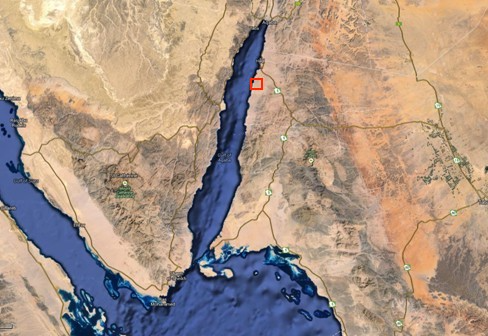
\includegraphics[width=0.9\textwidth, height=0.7\textwidth]{figures/chap04_field_data/golf_aqaba.png} 
               \caption{}
               \label{fig:golf_aqaba}
       \end{subfigure}%
       ~
       \begin{subfigure}[b]{.45\textwidth}
               \centering
               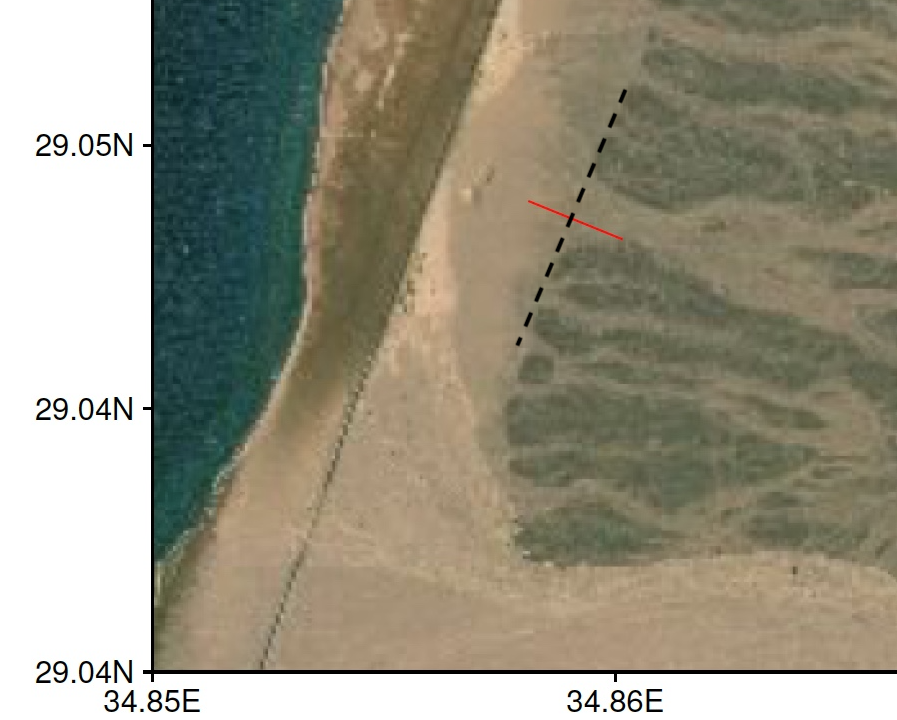
\includegraphics[width=0.9\textwidth,
               height=0.7\textwidth]{figures/chap04_field_data/location.png}
               \caption{}
               \label{fig:location}
       \end{subfigure}
       \caption{(a) A Google Earth satellite image showing the study area  (courtesy of  Sherif M. Hanafy, King Fahd University of Petroleum and Minerals). Red square at the eastern side of Gulf of Aqaba marks the location of the study area.  (b) Zoomed in view of the study area.  Blacked dashed line indicates the fault raptured at the 1995 earthquake. Red dashed line indicates the seismic profile.}
       \label{fig:golf_aqaba_location}
\end{figure}

\begin{figure}
 \centering
 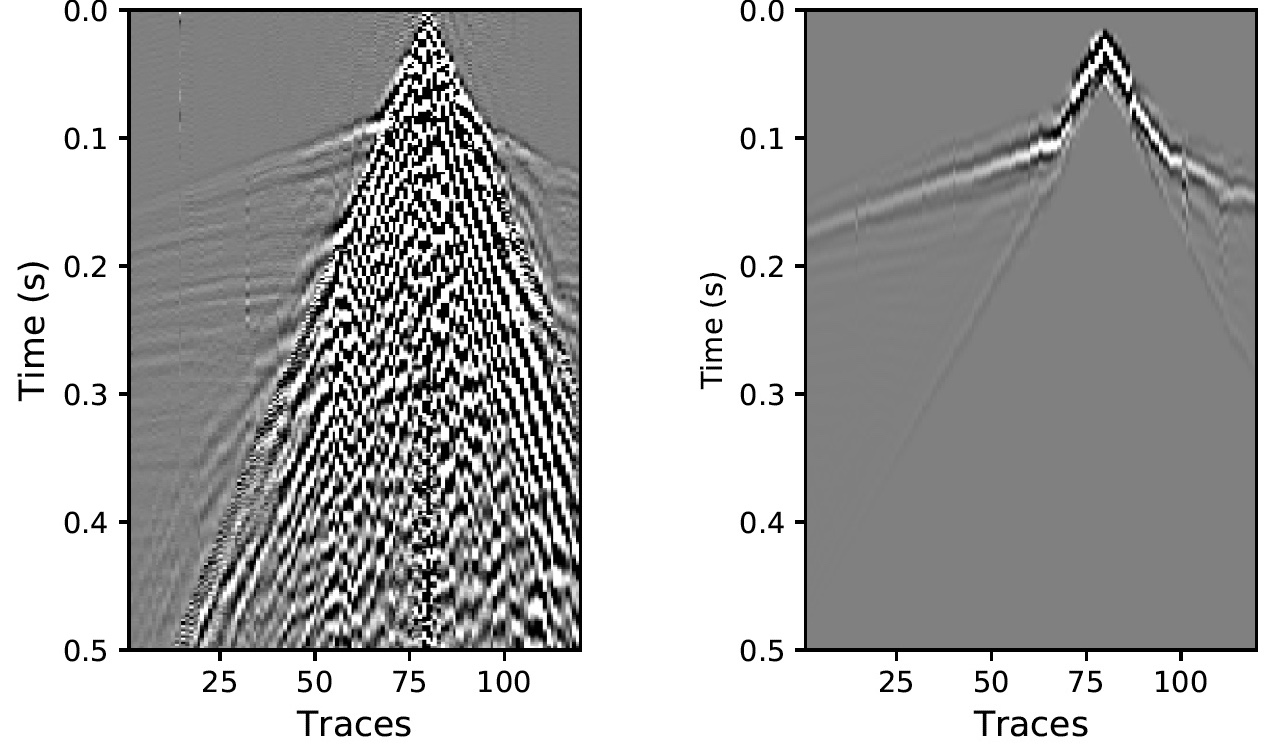
\includegraphics[width=0.9\textwidth]{figures/chap04_field_data/dataGulfAqaba} 
 \caption{ An example of a common shot gather (left), and processed of the gather showing the first arrival times (right).}
 \label{fig:shot_gather_fa}
\end{figure}